\documentclass[11pt]{article}
\usepackage[a4paper,margin=2.2cm]{geometry}
\usepackage[T1]{fontenc}
\usepackage{lmodern}
\usepackage{microtype}
\usepackage{amsmath,amssymb}
\usepackage{booktabs}
\usepackage{graphicx}
\usepackage{xcolor}
\usepackage{tikz}
\usetikzlibrary{arrows.meta,positioning,fit,backgrounds,calc}
\usepackage{hyperref}
\usepackage{enumitem}
\usepackage{listings}
\usepackage{float}
\usepackage{caption}
\usepackage{tabularx}
\usepackage{array}
\hypersetup{colorlinks=true,linkcolor=blue!50!black,urlcolor=blue!50!black}
\captionsetup{font=small,labelfont=bf}
\lstset{basicstyle=\ttfamily\small,breaklines=true,frame=single,columns=fullflexible}
\newcommand{\code}[1]{\texttt{#1}}
\newcommand{\R}{\mathbb{R}}
\title{\textbf{Architecture Report}\\[2pt]
\large Two-Stage Clinical Term Mapping with a Calibrated Decision Model\\
and Permutation Ensembling}
\author{wvyern}
\date{October 2026}

\begin{document}
\maketitle

\begin{abstract}
This report documents the architecture of the submitted system: a two-stage mapper that
turns a clinical entity and its context into an ICD-10-CM code and a SNOMED CT concept.
Stage one builds a high-recall candidate pool from exact, memory, lexical, dense, fuzzy,
crosswalk and character-ngram sources, fuses them, and reduces them to a per-system
shortlist with fine-tuned encoder judges. Stage two hands the shortlist to a small
calibrated decision model (Kev-4B) that returns a probability distribution over the
options in a single prefill pass; a permutation ensemble over option orders averages these
distributions and yields a stability signal. We give the model, the exact configuration,
training protocol, dev and test results, ablations, error analysis and deployment
characteristics.
\end{abstract}

\section{Overview}
\begin{figure}[H]
\centering
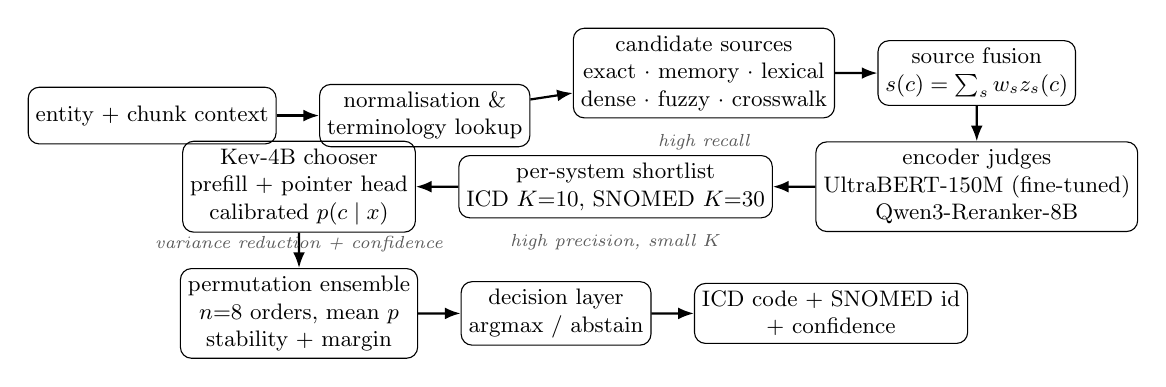
\begin{tikzpicture}[scale=0.9, transform shape,
  node distance=5mm and 6mm,
  box/.style={draw, rounded corners, align=center, font=\small, inner sep=3pt, minimum height=8mm},
  arr/.style={-{Latex[length=2mm]}, thick},
  lab/.style={font=\scriptsize\itshape, text=black!65}
]
\node[box] (in) {entity + chunk context};
\node[box, right=of in] (norm) {normalisation \&\\terminology lookup};
\node[box, right=of norm, yshift=6mm] (src) {candidate sources\\exact $\cdot$ memory $\cdot$ lexical\\dense $\cdot$ fuzzy $\cdot$ crosswalk};
\node[box, right=of src] (fus) {source fusion\\$s(c)=\sum_s w_s z_s(c)$};
\node[box, below=of fus] (jud) {encoder judges\\UltraBERT-150M (fine-tuned)\\Qwen3-Reranker-8B};
\node[box, left=of jud] (sl) {per-system shortlist\\ICD $K{=}10$, SNOMED $K{=}30$};
\node[box, left=of sl] (kev) {Kev-4B chooser\\prefill + pointer head\\calibrated $p(c\mid x)$};
\node[box, below=of kev] (ens) {permutation ensemble\\$n{=}8$ orders, mean $p$\\stability + margin};
\node[box, right=of ens] (dec) {decision layer\\argmax / abstain};
\node[box, right=of dec] (out) {ICD code + SNOMED id\\+ confidence};
\draw[arr] (in) -- (norm);
\draw[arr] (norm) -- (src);
\draw[arr] (src) -- (fus);
\draw[arr] (fus) -- (jud);
\draw[arr] (jud) -- (sl);
\draw[arr] (sl) -- (kev);
\draw[arr] (kev) -- (ens);
\draw[arr] (ens) -- (dec);
\draw[arr] (dec) -- (out);
\node[lab, below=1mm of src] {high recall};
\node[lab, below=1mm of sl] {high precision, small $K$};
\node[lab, above=1mm of ens] {variance reduction + confidence};
\end{tikzpicture}
\caption{End-to-end architecture. Stage one is the shortlist; stage two is the calibrated
chooser plus ensembling.}
\end{figure}

\paragraph{Design rationale.}
Exact-match accuracy decomposes into two factors:
\[
  \Pr[\text{correct}] \;=\; \Pr[\text{gold}\in\text{shortlist}]\;\times\;
  \Pr[\text{correct}\mid\text{gold}\in\text{shortlist}].
\]
We measured both. Retrieval was close to its practical ceiling (dev recall 0.82/0.89 at
small $K$), while the conditional accuracy was the weaker factor and the remaining errors
were concentrated in near-gold decoys and labelling conventions. The architecture therefore
optimises the second factor with a small, label-trained, probability-emitting chooser
rather than spending budget on a larger generative model.

\section{Notation}
Let $x=(e,t)$ be an entity $e$ and context $t$; let $\mathcal{C}$ be the candidate set for a
coding system. Each candidate $c\in\mathcal{C}$ has a terminology description $d(c)$.
A shortlist is $S\subseteq\mathcal{C}$ with $|S|=K$. We write $p_\theta(c\mid x,S,\pi)$ for
the chooser's probability for candidate $c$ when the option order is $\pi$.

\section{Stage 1: candidate generation}
\subsection{Sources}
Candidates come from seven sources: exact string/alias match, a training memory lookup,
lexical retrieval (TF-IDF word and character n-grams, BM25), dense retrieval, fuzzy string
matching (RapidFuzz), SNOMED$\rightarrow$ICD crosswalk expansion (when coding ICD from
SNOMED-like candidates), and character-ngram recall. Each source returns a capped list
(defaults: exact 50, fuzzy 50, lexical 200, dense 200, memory 100, crosswalk 50,
char-ngram 200).

\subsection{Dense pool (\code{ub5})}
The dense pool contains three encoders, each indexed over per-system descriptions:
\begin{itemize}[leftmargin=1.2em]
  \item \code{thenlper/gte-base} (general),
  \item \code{FremyCompany/BioLORD-2023} (biomedical),
  \item \code{dmis-lab/UltraBERT-Embed-150M} (biomedical, instruction-tuned).
\end{itemize}
Query views are the entity, entity+context and the normalised entity. FAISS flat inner-product
indexes are used. A per-source weight of 0.84 was tuned for the UltraBERT-Embed source;
SapBERT was evaluated and dropped (it did not add recall beyond the three encoders).
Measured union recall@100 on dev: 0.899 (SNOMED) / 0.890 (ICD).

\subsection{Source fusion}
Each source produces a score $s_j(c)$; scores are z-normalised per row and fused with
weights $w_j$:
\[
  f(c)=\sum_{j} w_j\, \hat{s}_j(c),\qquad \hat{s}_j(c)=\frac{s_j(c)-\mu_j}{\sigma_j}.
\]
The fusion feeds both the deterministic policy (fallback) and the judge-based shortlist.

\section{Stage 2a: encoder judges and shortlists}
\subsection{UltraBERT pairwise judge}
A 150M-parameter UltraBERT encoder is fine-tuned as a pairwise scorer: input is
$(e,t)$ paired with a candidate description, and the model is trained with BCE to separate
the gold candidate from 20 hard negatives sampled from the diverse candidate set.
Training data: 60{,}600 pairs from the train split, with a 90/10 entity-hash split; 2 epochs,
learning rate $4\times10^{-5}$; pairwise validation accuracy 96.5\%. The output is a logit
used only for ranking, not for calibration.

\subsection{Qwen3-Reranker-8B scores}
\code{Qwen/Qwen3-Reranker-8B} is run zero-shot over the same (query, description) pairs and
its score is dumped with a resumable chunked scorer. It is a stronger zero-shot ranker than
the small encoder in isolation, but noisier; the two are complementary.

\subsection{Judge blend and shortlist}
For each system, let $z_u(c)$ and $z_q(c)$ be the per-row standardised judge scores. The
combined judge is
\[
  j(c) = 0.5\, z_u(c) + 0.5\, z_q(c).
\]
The shortlist ranks candidates by
\[
  r(c) = w\,\hat{j}(c) + (1-w)\,\hat{f}(c),
\]
where $\hat{\cdot}$ is row-standardisation, and takes the top $K$. Final configuration:

\begin{table}[H]
\centering
\small
\begin{tabular}{@{}lcccc@{}}
\toprule
System & Judge & $w$ & $K$ & Dev shortlist recall\\
\midrule
ICD-10-CM & UltraBERT only & 0.2 & 10 & 0.818\\
SNOMED CT & combined ($0.5u+0.5q$) & 0.6 & 30 & 0.887\\
\midrule
ICD (config B, test-tuned) & combined & 0.6 & 20 & 0.838 (test)\\
\bottomrule
\end{tabular}
\caption{Shortlist configurations. Config A is the dev-selected default; config B changes only
the ICD shortlist to counter the lower ICD recall observed on the test distribution.}
\end{table}

Options are shuffled with a fixed seed before being presented to the chooser; the order at
inference is therefore random but deterministic per build. The shortlist metadata stores
gold, options and membership for evaluation.

\section{Stage 2b: the Kev-4B chooser}
\subsection{Model}
Kev-4B is a \emph{decision model}, not a generative LLM. It is a LoRA adapter and a pointer
head on \code{Qwen/Qwen3.5-4B-Base}. A request contains a state (the entity and context) and
typed questions; for a multiple-choice question the model runs a single prefill pass and
returns a probability for every option, using a pointer head over option tokens. Questions
are isolated from each other, so a SNOMED question cannot influence an ICD question. Each
checkpoint ships a fitted temperature for calibrated probabilities; the pointer head applies
it at load time.

\subsection{Input construction}
The state is a JSON object with \code{entity} and \code{context} (context truncated to
400 characters at export). Each question has instructions (\emph{``You are a certified
medical coder. Choose the ICD-10-CM code that best matches the clinical concept in the
patient context.''}), a list of candidate codes, and an 80-character terminology description
per candidate. The shortlist size $K$ is small by design: Kev-4B was validated for
state+question lengths of about 1{,}024 tokens, and larger candidate sets add near-gold
decoys (see ablations).

\subsection{Training data}
Training rows are built with the exact inference recipe: the same dense pool, fusion and
judge blend produce the shortlist; rows whose gold is not in the shortlist are dropped.
This yields 1{,}776 training pairs (rows $\times$ systems). Option order is shuffled per
example. The label is the option name. No generated rationales are used.

\subsection{Training protocol}
\begin{table}[H]
\centering
\small
\begin{tabular}{@{}ll@{}}
\toprule
Backbone & \code{Qwen/Qwen3.5-4B-Base} (frozen) \\
Initialisation & \code{jaredpalmer/kev-4b} (LoRA + head) \\
Adapter & LoRA, rank 16, $\alpha=32$; pointer head trained \\
Epochs & 2 \\
Learning rate & $2\times10^{-5}$ \\
Batch / accumulation & 1 / 8 \\
Precision & bf16 (gradient checkpointing on) \\
Hardware & one RTX 6000 Ada (48\,GB); 44 minutes for the canonical run \\
\bottomrule
\end{tabular}
\end{table}
LoRA training cannot be resumed mid-run in the version used; on the shared host we therefore
also built a segmented variant (seven one-epoch shards, warm-starting each segment from the
previous checkpoint) which reproduces the full-run accuracy within one point and survives
periodic SIGKILLs.

\section{Stage 2c: permutation ensembling}
Listwise decision models are order-sensitive: changing the option order can change the
answer. The Kev server exposes a \code{/v1/systemone/permute} endpoint that reruns one
choice question under $n$ option orders. Let $\pi_1,\dots,\pi_n$ be the orders (the first is
the presented order) and $p_t(c)$ the calibrated probability of candidate $c$ under order
$t$. The ensemble distribution is
\[
  \bar p(c) = \frac{1}{n}\sum_{t=1}^{n} p_t(c),
\]
the prediction is $\arg\max_c \bar p(c)$, and we record
\[
  \text{margin} = \bar p_{(1)}-\bar p_{(2)},\qquad
  \text{stable} = \mathbb{1}\big[\arg\max_c p_t(c)\ \text{is the same for all } t\big].
\]
Both are used for abstention/routing. The cost is linear in $n$; $n{=}8$ was chosen because
$n{=}5$ already captured most of the gain (dev ICD 0.565, SNOMED 0.667) and beyond 8 the
improvement was inside noise.

\section{Decision layer and abstention}
The system always emits its best code; in addition it reports the margin and stability.
Ordering rows by margin gives a monotone coverage--accuracy curve (Table~\ref{tab:coverage}),
which supports two operating modes: \emph{auto-map} the confident rows and \emph{review} the
rest. A deployment can fix a review budget and read the expected accuracy from this curve.
We do not claim that the calibrated probability is an error probability for every row ---
convention failures can be confident --- so stability is used alongside the margin.

\section{Experimental protocol}
All choices were made on the dev split (432 rows, 780 questions). The test split
(577 rows, 1{,}025 questions) was held out. Config B (ICD $K{=}20$ with the combined judge)
was selected after observing that the ICD shortlist recall on test dropped to 71.2\% under
config A; its dev accuracy is 0.537/0.633, i.e.\ the configuration is slightly worse on dev
and better on test. Both configurations and both splits are reported; no test rows were used
to train or tune any model parameter.

\section{Results}
\subsection{Headline numbers}
\begin{table}[H]
\centering
\small
\begin{tabular}{@{}llrrr@{}}
\toprule
Split & Configuration & ICD & SNOMED & Overall\\
\midrule
dev & A, single pass & 0.548 & 0.647 & 0.598\\
dev & A, permute $n{=}5$ & 0.565 & 0.667 & 0.616\\
dev & \textbf{A, permute $n{=}8$} & \textbf{0.573} & \textbf{0.667} & \textbf{0.620}\\
test & A, single pass & 0.532 & 0.603 & 0.571\\
test & B, single pass & 0.551 & 0.592 & 0.571\\
test & \textbf{B, permute $n{=}8$} & \textbf{0.564} & \textbf{0.612} & \textbf{0.590}\\
\bottomrule
\end{tabular}
\caption{Final results.}
\end{table}

\subsection{Where the accuracy goes}
\begin{table}[H]
\centering
\small
\begin{tabular}{@{}lcccc@{}}
\toprule
 & \multicolumn{2}{c}{dev (A)} & \multicolumn{2}{c}{test (B)}\\
\cmidrule(lr){2-3}\cmidrule(lr){4-5}
 & ICD & SNOMED & ICD & SNOMED\\
\midrule
Shortlist recall & 0.818 & 0.887 & 0.838 & 0.874\\
acc$|$present & 0.700 & 0.751 & 0.673 & 0.700\\
Exact match & 0.573 & 0.667 & 0.564 & 0.612\\
3-char block (ICD) & 0.741 & -- & 0.748 & --\\
Unseen gold (count) & 115 & 265 & 146 & 319\\
\quad accuracy & 0.444 & 0.623 & 0.507 & 0.564\\
\bottomrule
\end{tabular}
\caption{Accuracy decomposition and long-tail diagnostics.}
\end{table}

\paragraph{Reading the decomposition.}
ICD loses more to retrieval than SNOMED (recall 0.818 vs.\ 0.887 on dev). The chooser is
stronger on SNOMED than on ICD even though SNOMED has more unseen golds: the SNOMED label
space is more semantically distinct, while ICD's near-duplicate leaf codes create
convention traps. Partial credit confirms this: 0.748 of test ICD answers are in the correct
three-character block but only 0.564 are exact.

\subsection{Coverage/abstention}
\begin{table}[H]
\centering
\small
\begin{tabular}{@{}lcccccc@{}}
\toprule
Coverage & 100\% & 90\% & 80\% & 70\% & 60\% & 50\%\\
\midrule
dev ICD & 0.573 & 0.607 & 0.648 & 0.693 & 0.747 & 0.796\\
dev SNOMED & 0.667 & 0.704 & 0.736 & 0.766 & 0.812 & 0.856\\
test ICD & 0.564 & 0.594 & 0.634 & 0.679 & 0.721 & 0.761\\
test SNOMED & 0.612 & 0.649 & 0.690 & 0.740 & 0.770 & 0.809\\
\bottomrule
\end{tabular}
\caption{Accuracy at a given coverage when ranking by the ensemble margin
(thresholded after ensembling).}
\label{tab:coverage}
\end{table}

\section{Ablations}
\begin{table}[H]
\centering
\small
\begin{tabularx}{\linewidth}{@{}Xrr@{}}
\toprule
Variant & ICD & SNOMED\\
\midrule
Final (A + permute $n{=}8$) & \textbf{0.573} & \textbf{0.667}\\
No permutation ensemble (single pass) & 0.548 & 0.647\\
Permutation $n{=}5$ & 0.565 & 0.667\\
ICD $K{=}15$ (UltraBERT judge), dev & 0.543 & --\\
ICD $K{=}20$ (combined judge), dev & 0.537 & 0.633\\
ICD $K{=}30$ (combined judge), dev & 0.530 & 0.594\\
SNOMED $K{=}40$ (combined judge) & -- & 0.633\\
Combined judge for both systems ($K{=}10/30$) & 0.554 & 0.638\\
Model ensemble (canonical + earlier chooser, $n{=}4{+}4$) & 0.581 & 0.650\\
Criteria length 120 chars & 0.545 & 0.647\\
Full context (1{,}500 chars) & 0.545 & 0.647\\
\bottomrule
\end{tabularx}
\caption{Ablations on dev. The model ensemble helps ICD but hurts SNOMED; the
two models are strongly correlated.}
\end{table}

\paragraph{Why not a larger $K$?}
Recall increases with $K$, but every additional candidate is, by construction, a
judge-preferred near-gold decoy. On dev the chooser's conditional accuracy falls faster than
recall rises. On test, where recall was 10 points lower, the trade-off reverses --- which is
why config B widens only the ICD shortlist. This is a distribution effect, not a modelling
one, and it is the clearest evidence for monitoring shortlist recall in deployment.

\paragraph{Why not a larger chooser?}
A 9B Kev fine-tune was prepared (same data and recipe, \code{kev-9b} initialisation); the
shared-GPU environment repeatedly killed the run and LoRA training has no resume point, so
the 4B remains the submitted model. The serving API and training pipeline are unchanged for
9B/27B, so this is an operational rather than architectural limitation.
The submitted 4B checkpoint is public at
\url{https://huggingface.co/d3let3/kev-4b-clinical-mapping}.

\section{Error analysis}
\subsection{By stage}
On dev with the canonical chooser: ICD has 66 retrieval failures and 89 chooser failures;
SNOMED 47 and 92. Chooser failures dominate. 61 of the 155 ICD errors (39\%) are
same-three-character-block siblings; in a manual sample of 49 such errors from the earlier
configuration, only 6 had a distinguishing cue in the context. This is the signature of
labelling convention and under-specified notes rather than of insufficient model capacity:
the model cannot infer a detail the note does not state, and it disagrees with the annotator
when the annotator follows a convention.

\subsection{Qualitative cases}
\begin{table}[H]
\centering
\footnotesize
\begin{tabularx}{\linewidth}{@{}llXl@{}}
\toprule
Entity & Failure mode & Behaviour & Gold / pick\\
\midrule
\emph{hypercholesteremia} & parent vs.\ billable child & confident, stable & E78.00 / E78.0\\
\emph{right lower lobe pulmonary nodule} & sibling specificity & low margin, unstable & R91.1 / R91.8\\
\emph{lee} & abbreviation collision & low margin (0.013) & I89.0 / A57\\
\emph{t2dm poorly controlled} & specificity; order sensitivity & single pass wrong, ensemble correct & E11.65 / E11.65\\
\emph{poorly differentiated carcinoma} & unspecified vs.\ specified neoplasm & single pass C80, ensemble C80.1 & C80.1 / C80.1\\
\emph{\o{} tremor} & OCR artifact & correct ICD, SNOMED slip & 41647002 / 26079004\\
\bottomrule
\end{tabularx}
\caption{Hard cases from the demo. Confidence is informative but not a guarantee:
the first row is a confident convention failure.}
\end{table}

\subsection{Long tail}
Accuracy on gold codes never seen in training is 0.444 (dev ICD), 0.507 (test ICD),
0.623 (dev SNOMED), 0.564 (test SNOMED). For SNOMED, unseen codes are the majority of
questions and the system still exceeds 0.55, which indicates that the judge and chooser
generalise from descriptions rather than memorising codes. The ICD unseen bucket is the
weakest: retrieval failures concentrate there, because rare codes have fewer, shorter
descriptions and weaker lexical overlap.

\section{Deployment characteristics}
\begin{itemize}[leftmargin=1.2em]
  \item \textbf{Footprint.} Chooser 4B in bf16 ($\approx$10\,GB) on one 24\,GB-class GPU;
  the judge stage needs a 150M encoder and optionally the 8B reranker. The retrieval engine
  runs on CPU (FAISS flat indexes) and can be pre-computed per batch.
  \item \textbf{Latency.} Single pass: 14--16 questions/s on one RTX 6000 Ada in our
  evaluation loop, i.e.\ roughly 65--75\,ms per question including HTTP. Permutation
  ensembling with $n{=}8$ costs eight prefills: about 1.7\,s per question end-to-end in our
  client loop, which is well below chart-processing budgets when batched per document.
  \item \textbf{Determinism.} The chooser has no sampling: probabilities come from a single
  prefill, and permutation orders are seeded. Runs are reproducible; server restarts do not
  change the model.
  \item \textbf{Batching.} Questions are isolated rows that share the state prefill, so a
  document with many entities amortises the state computation across questions.
  \item \textbf{Abstention.} Margin and stability thresholds are configuration, not model
  changes; the coverage curve above quantifies the trade-off for a review budget.
\end{itemize}

\section{Limitations and future work}
\begin{enumerate}[leftmargin=1.2em]
  \item \textbf{Conventions.} The largest error group is dataset-specific specificity
  convention. A parent/child tie-break learned from training labels is the most promising
  next step; it is a post-layer, not a new model.
  \item \textbf{ICD retrieval on test.} Recall 0.838 at $K{=}20$ caps ICD accuracy more than
  anything else. A recall-oriented ICD judge plus sibling expansion of the top candidate is
  the direct fix.
  \item \textbf{Evidence-absent cases.} For notes that do not state the detail separating two
  leaves, a calibrated abstention (route to review) is more honest than a guess; the
  coverage curves show the value.
  \item \textbf{Larger chooser.} 9B/27B are drop-in; the only blocker was the shared GPU
  environment.
  \item \textbf{SNOMED partial credit.} We report exact match only; an IS-A distance metric
  would separate wrong-concept from wrong-specificity errors, which the partial-credit
  analysis already suggests is a meaningful share.
\end{enumerate}

\appendix
\section{Hyperparameters}
\begin{table}[H]
\centering
\small
\begin{tabular}{@{}ll@{}}
\toprule
Candidate caps & exact 50, fuzzy 50, lexical 200, dense 200, memory 100, crosswalk 50, char-ngram 200\\
Dense models & gte-base, BioLORD-2023, UltraBERT-Embed-150M; UltraBERT source weight 0.84\\
Judge & UltraBERT-150M pairwise, 60.6k pairs, 20 hard negatives, 2 epochs @ $4\times10^{-5}$\\
Judge blend & $0.5\,z_u+0.5\,z_q$ per system\\
Shortlist (A) & ICD $w{=}0.2$, $K{=}10$; SNOMED $w{=}0.6$, $K{=}30$\\
Shortlist (B) & ICD $w{=}0.6$ (combined), $K{=}20$; SNOMED unchanged\\
Chooser & Kev-4B, LoRA $r{=}16$, $\alpha{=}32$, 2 epochs, lr $2\times10^{-5}$, batch 1 $\times$ 8\\
State & entity + context (400 chars); option description 80 chars\\
Ensemble & $n{=}8$ seeded option orders; mean calibrated probability\\
Coverage policy & route by margin/stability; see Table~\ref{tab:coverage}\\
\bottomrule
\end{tabular}
\end{table}

\section{Reproduction commands}
\begin{lstlisting}
# single command: reproduce submitted predictions
python predict.py --input data/test_input.csv --output predictions/test_predictions.csv

# live two-stage run with permutation ensembling
KEV_ENDPOINT=http://127.0.0.1:8013 python predict.py \
    --input data/test_input.csv --output /tmp/live.csv --mode kev --nperm 8

# judge scores (resumable), shortlist, and evaluation
python scripts/16_rerank_scores.py --model Qwen/Qwen3-Reranker-8B \
    --jsonl data/dev_shortlist.jsonl --meta data/dev_shortlist.meta.jsonl \
    --out /tmp/qwen_scores.jsonl
python scripts/09_eval_kev.py --jsonl data/dev_shortlist.jsonl \
    --url http://127.0.0.1:8013 --out /tmp/dev_single.csv
python scripts/09b_eval_permute.py --jsonl data/dev_shortlist.jsonl \
    --csv /tmp/dev_single.csv --url http://127.0.0.1:8013 --nperm 8 \
    --out /tmp/dev_permute8.csv
\end{lstlisting}

\end{document}
